\subsection{Route Reliability Computation}
In the following experiments, we apply the techniques for computing
\textit{pltts} to the approaches discussed in \cref{sec:methods}. The first goal
is to evaluate the impact of choosing the right pltt computation technique on
the accuracy of the route pmf. In addition we will assess the effectiveness of
considering the attributes used to classify route computation algorithms in
\cref{sec:methods}.

For these experiments, we use 10 different paths, spanning the road network in
\ref{subsec:Dataset}. The selected paths are 45 miles on average, consisting of
approximately 40 edges. For each path, we use the same standard \textit{start
times} we used for the link travel time predictions. Again, we build a model
with each approach using data from model days and compare the accuracy of the
model with the actual travel time during the test days. Finally, when using the
pltt computation techniques, we only use the optimal parameter discovered in
\cref{subsec:pltt_prediction} for each technique.

\begin{figure}
    \centering
    \subfigure[ConStaInd]{
        \label{fig:ConStaInd}
        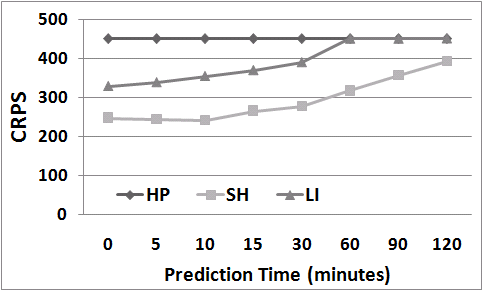
\includegraphics[width = 0.4\columnwidth]{figures/Approaches_ConStaInd.png}
    }
    \subfigure[DisStaInd]{
        \label{fig:DisStaInd}
        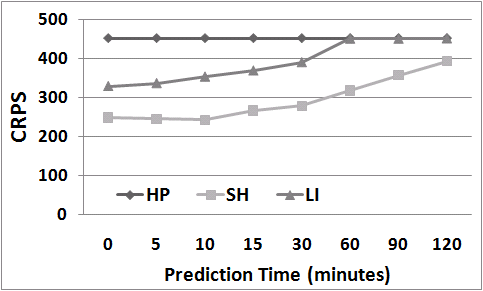
\includegraphics[width = 0.4\columnwidth]{figures/Approaches_DisStaInd.png}
    }
    \subfigure[DisTimInd]{
        \label{fig:DisTimInd}
        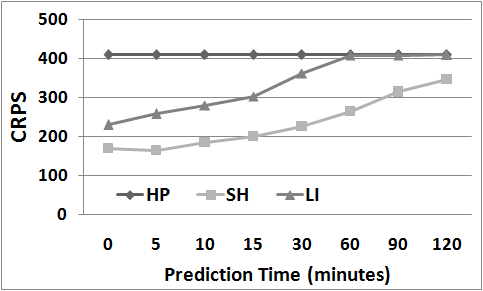
\includegraphics[width = 0.4\columnwidth]{figures/Approaches_DisTimInd.png}
    }
    \subfigure[ConStaCor]{
        \label{fig:ConStaCor}
        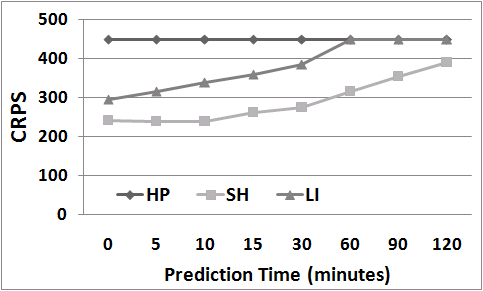
\includegraphics[width = 0.4\columnwidth]{figures/Approaches_ConStaCor.png}
    }
    \caption{Applying pltt computation techniques to route computation algorithms}
    \label{fig:route_pltt}
\end{figure}

As we can see in \cref{fig:route_pltt}, depending on how we model the link travel times, the accuracy of the route pdf (\textbackslash pmf) can vary. Comparing \cref{fig:route_pltt} and \cref{fig:all_results} shows that the accuracy of pltt models \textbf{directly} impact the accuracy of route pmfs. In fact, applying a \textit{good} pltt model to a \textit{bad} route model can yield more accurate models than applying a \textit{bad} pltt model to a \textit{better} route model.

\begin{figure}[h]
	\centering
	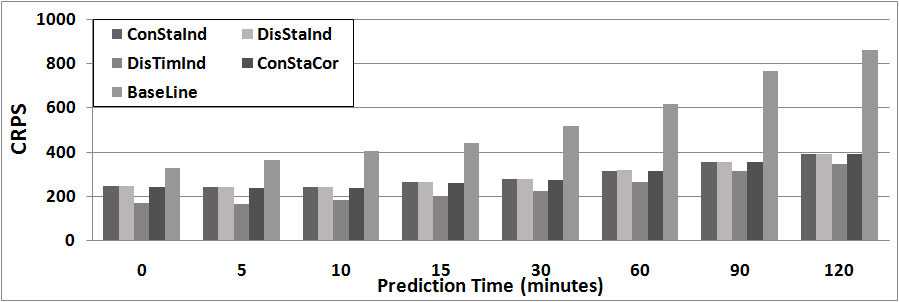
\includegraphics[width = 0.9\columnwidth]{figures/Approaches_All.png}
	\caption{CRPS for probabilistic path computation}\label{fig:path_comp}
\end{figure}

In \cref{fig:path_comp} we put the results of applying the SH approach (\cref{subsec:SH}) to each route computation algorithm side by side. Several observations can be derived from this experiment:

\begin{itemize}
\item Comparing ConStaInd and DisStaInd, we can observe the same characteristics we observed for single links. Representing the link travel times trough a \textit{pmf} or a normal distribution does not drastically change the accuracy of the travel time prediction.
\item  Considering the time-dependency (DisTimInd) however, has a very positive effect on the prediction accuracy, where the results are up to 25\% better compared to the time-independent approaches which have otherwise the same characteristics.
\item The ConStaCor approach is again time-independent and it seems that the consideration of correlation between links does only yield a marginal improvement over the same approach without correlation (ConStaInd). In our experiments, we observe only a 1\%-2\% improvement through the incorporation of correlation in this setting.
\end{itemize}

As an additional comparison partner we included an approach that is used in current route planing systems, named \textit{Baseline}. \textit{Baseline} uses the situation at the \textit{query time} and computes the path travel time without prediction based on the currently available deterministic travel times. The outcome will consequently be a non-probabilistic value as well. The CRPS method allows us to directly compare this approach to the probabilistic counterparts, since it converges to the mean error in the case of certain predictions (i.e., the CRPS can be interpreted as the difference of the prediction and the true value in seconds). The results show that under all settings the probabilistic approaches are superior to the \textit{Baseline} approach which once more justifies the use of probabilistic models in this application.

\begin{figure}
    \centering
    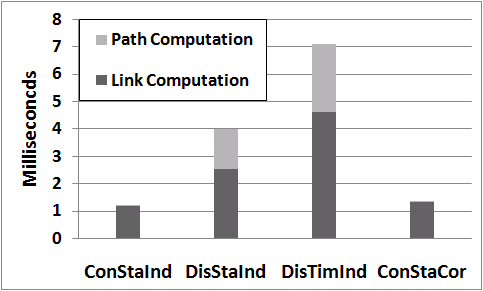
\includegraphics[width = 0.75\columnwidth]{figures/Runtime.png}
    \caption{Runtimes}\label{fig:runtimes}
\end{figure}

Lastly, we evaluated the runtime of all path computation methods discussed in Section \ref{sec:methods}. Runtimes are broken into link travel time prediction and path computation in Figure \ref{fig:runtimes}. Generally, the continuous approaches perform much better due to the analytical nature which yields a much better runtime complexity. As expected, the more complexity we add to the approaches based on a discrete representation, the more costly in terms of computation they become. Link travel time prediction and path computation contribute rather equivalent portions to the runtime in all approaches.